\chapter{Compact Muon Solenoid Experiment
\label{ch:cmsexperiment}}
\setcounter{section}{-1}

The Compact Muon Solenoid (CMS) experiment is one of two general-purpose detectors at the LHC. It is located about 100\unit{m} underground at Point 5 of the LHC ring, near Cessy, France. The detector is cylindrically shaped, with total length 22\unit{m}, diameter 15\unit{m}, and weight 14000\unit{tons}. Figure \ref{fig:cms-overall} shows the overall layout of the detector.

\begin{figure}[hbt]
\begin{center}
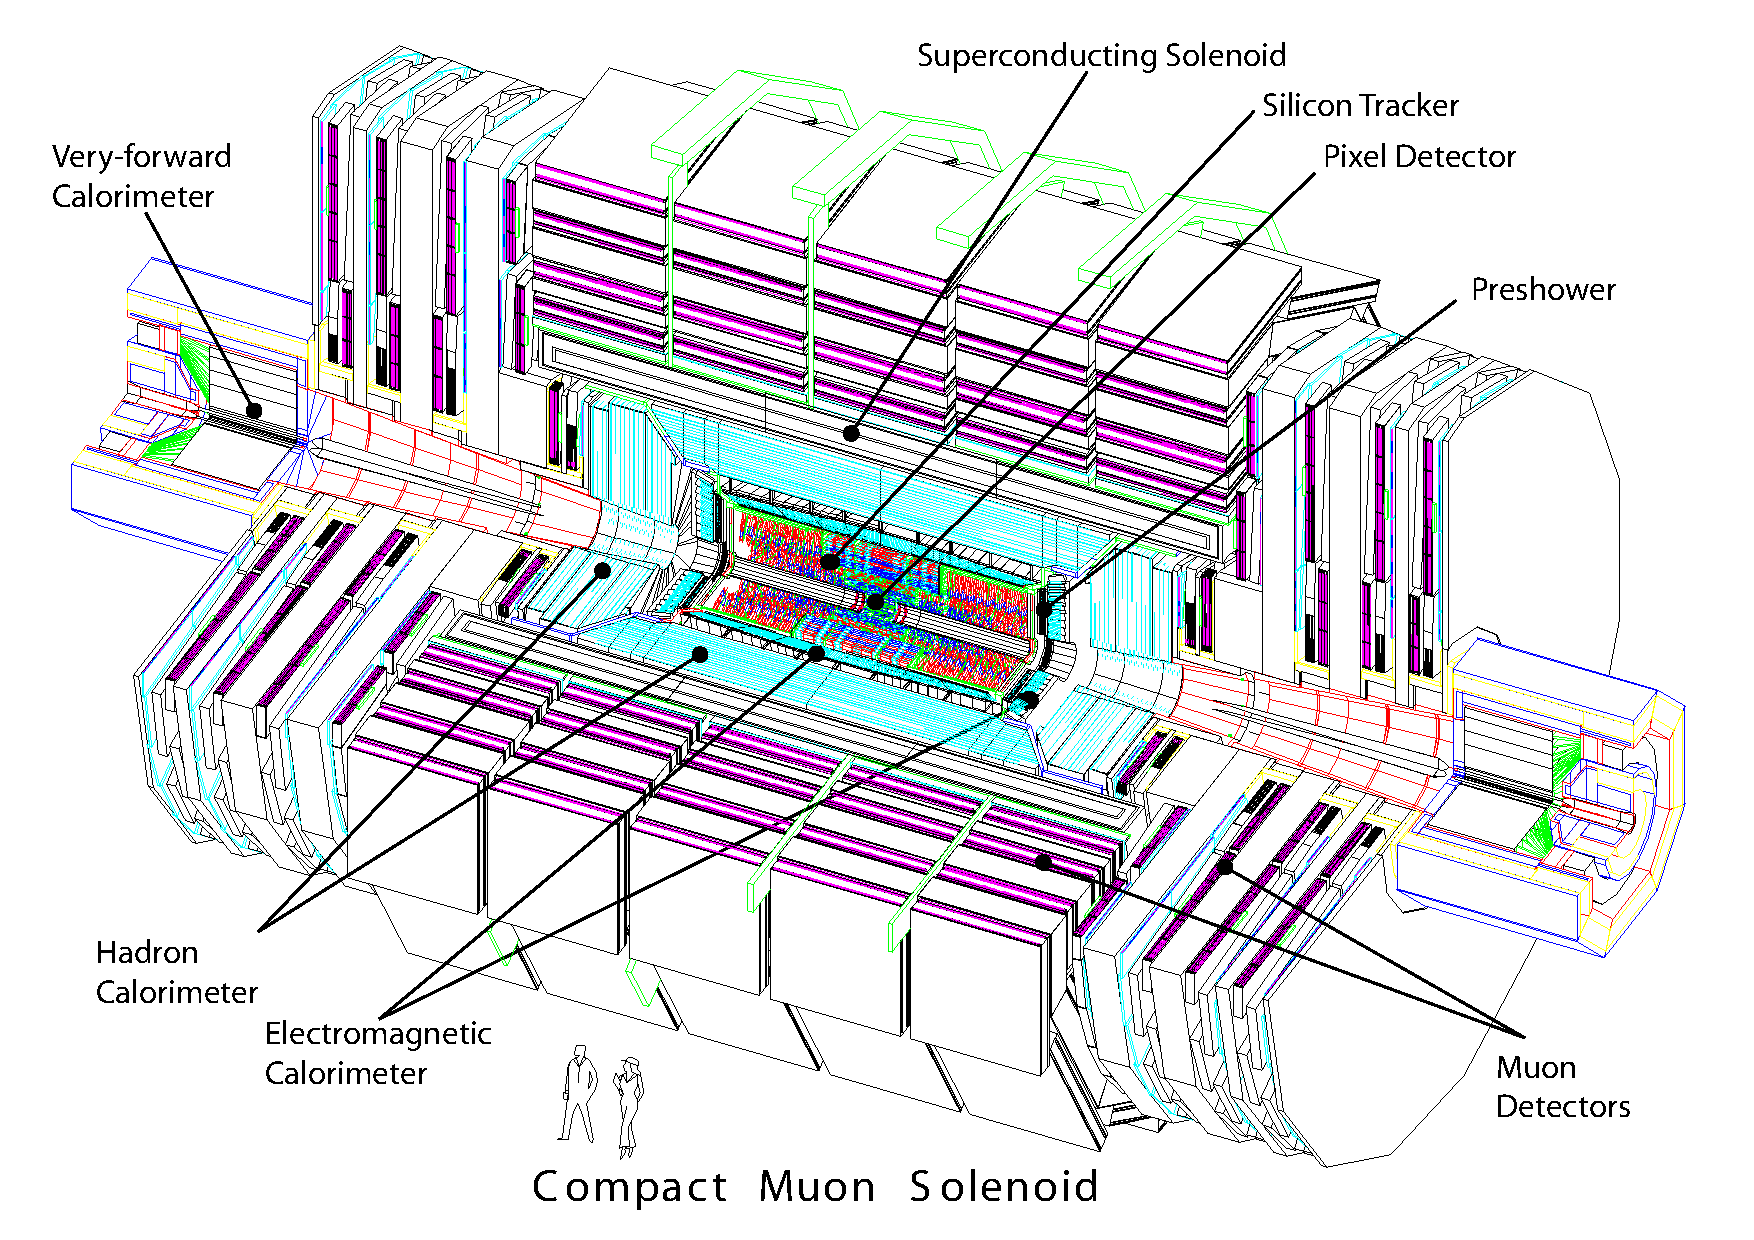
\includegraphics[width=0.95\textwidth]{figures/cms_complete_labelled.pdf}
\caption{The layout of the CMS detector, with the subdetectors labeled and two humans shown for a height reference.}
\label{fig:cms-overall}
\end{center}
\end{figure}

The center of the detector is used as the origin of the right-handed coordinate system that describes locations and directions within the detector. The $z$-axis is assigned to the direction of the LHC beam line, pointing anti-clockwise in the direction of Beam 2. The polar angle $\theta$ is defined as the angle away from the positive $z$-axis. This angle is often transformed into pseudorapidity, defined as $\eta = -\text{ln}[\text{tan}(\theta/2)]$, which has several desirable properties. It is independent of the particle mass and energy, and it is approximately equal to the rapidity for relativistic particles. Differences in pseudorapidity are Lorentz invariant for boosts in the $z$ direction, and particle production is approximately uniform in $\eta$.

The plane transverse to the $z$-axis comprises the $x$- and $y$-axes, with the $x$-axis pointing toward the center of the LHC ring and the $y$-axis pointing upward in the normal direction. The azimuthal angle $\phi$ is defined as the angle away from the positive $x$-axis in the transverse plane, and the radial coordinate $r$ is defined as the distance from the origin in the transverse plane. The magnitude of the component of momentum in the transverse plane is labeled \pt. The total transverse momentum of every event must be conserved, so the negative vector sum of \vecpt for all particles in the event is defined as the missing transverse momentum: $\vecmet = - \sum_{i} \vecpt^{(i)}$. The magnitude of this quantity is called the missing transverse energy, denoted as \met.

As a general purpose detector, the CMS experiment detects all long-lived SM particles, except neutrinos, which can only be measured by omission in the transverse plane via \met. These particles can be categorized as electrons, photons, muons, charged hadrons, and neutral hadrons. The latter two categories are usually found grouped into cones called jets, and can originate from gluons, light quarks, bottom quarks with displaced vertices, or hadronically decaying tau leptons. The identification of particles and related objects with the CMS detector is described in more detail in Ch. \ref{ch:reconstruction}.

The CMS detector must measure these particles with sufficient accuracy to accomplish the experiment's physics goals, imposing requirements which are met by the combination of the CMS subdetectors. The inner tracker measures event vertices and charged-particle momentum, with the help of the superconducting solenoid. The measurement of muon momentum is supplemented by the muon system. The electromagnetic calorimeter measures electron and photon energy, and the hadron calorimeter measures the energy from charged and neutral hadrons. In addition, the LHC operates at a high instantaneous luminosity, approaching $1\times10^{34}\percms$; with an expected proton-proton cross section of 100\unit{mb} at the LHC center-of-mass energies, the collision rate is approximately 1\unit{MHz}. To cope with this incredibly high collision rate, the CMS experiment employs a trigger system to select interesting events at a rate which can be stored and processed by the computing systems. The delivered luminosity is also measured by the detector, using special techniques. The following sections describe the LHC, based on Ref. (blah), and the CMS subdetector systems, based on Ref. \cite{CMSJINST}.

\section{The Large Hadron Collider}

\section{Tracker}

\section{Electromagnetic Calorimeter}

\section{Hadron Calorimeter}

\section{Solenoid}

\section{Muon System}

\section{Trigger}

\section{Luminosity Measurement}